%% IMPORTANT: Once working, run latex 3 times to get listoffigures to work

%% Be sure to check spelling!

%% Put **your** name and the proper due date in place

%% Copy the lstlisting and figure code as many times as you need
%% Be sure to put in your own file names if appropriate

%% Note that the \epsfig commands are currently commented out - until the
%%%% files exist, processing this code without them will result in an error
%%%% so leave the comments until you have created the graphics files!

\documentclass{article}
\usepackage{amsmath}    % loads AMS-Math package
\usepackage{epsfig}     % allows PostScript files
\usepackage{listings}   % allows lstlisting environment
\usepackage{moreverb}   % allows listinginput environment
\usepackage[letterpaper, margin=0.75in]{geometry}  % set paper size/margins

\begin{document}
\begin{center}
\rule{6.5in}{0.5mm}\\~\\
\textbf{\large EGR 103L -- Fall 2017}\\~\\
\textbf{\huge Laboratory 2 - Introduction to MATLAB\\
Solutions}\\~\\
Ian Hanus (ih52)\\
Lab Section 1, Tuesday 8:30-11:30\\
September 17, 2017\\~\\
{\small I understand and have adhered to all the tenets of the Duke
  Community Standard in completing every part of this assignment.  I
  understand that a violation of any part of the Standard on any part
  of this assignment can result in failure of this assignment, failure
  of this course, and/or suspension from Duke University.} 
\rule{6.5in}{0.5mm}\\
\end{center}
\tableofcontents
\listoffigures
\pagebreak

\section{Introduction}
% Add your introduction here
The program created takes inputs of mass in kilograms and converts it into force in Newtons by multiplying by 9.81. It then takes inputs of displacement in inches and converts these to displacement in meters. The program then plots the points with the force as the independent variable and the corresponding displacements as the dependent variable. A best fit line for a first order polynomial is found and graphed along with the data points. Then 100 representational force values are created between the minimum and maximum forces and used to predict displacement. Next the slope and y-intercept of the best fit line are  measured which, according to the equation Displacement $=$ Compliance$*$Force $+$ Initial Displacement, means compliance is equal to the slope and initial displacement is equal to the y-intercept. Then, looking at the graphs for each data set, one can tell if the line fits the data well which determines if the beam is acting as a spring.

\section{Data Obtained}
The three data sets from the experiments are presented in Table
\ref{DataTables}.
% replace the tables below with *your* data sets.  You may cut and paste
% from the MATLAB window and then add \\ and & as needed

\renewcommand{\arraystretch}{1.4}
\begin{table}[h]
\begin{center}
\begin{tabular}{ccc}
\begin{tabular}[t]{|c|c|}\hline
\multicolumn{2}{|c|}{Beam1.dat}\\ \hline
\textbf{Mass} & \textbf{Disp.}\\
(kg) & (in)\\ \hline
         
            0 & 4.0908e-01\\
   2.4018e-01 & 5.1145e-01\\
   4.8037e-01 & 1.1085e+00\\
   7.2055e-01 & 1.6810e+00\\
   9.6073e-01 & 2.2016e+00\\
   1.2009e+00 & 2.5752e+00\\
   1.4411e+00 & 3.0958e+00\\
   1.6813e+00 & 3.5045e+00\\
   1.9215e+00 & 4.1159e+00\\
   2.1616e+00 & 4.4975e+00\\ \hline
\end{tabular}
&
\begin{tabular}[t]{|c|c|}\hline
\multicolumn{2}{|c|}{Beam2.dat}\\ \hline
\textbf{Mass} & \textbf{Disp.}\\
(kg) & (in)\\ \hline
            0 &  1.4446e-01\\
   2.4969e-01 & 4.5522e-02\\
   4.9939e-01 & 1.1184e-01\\
   7.4908e-01 & 2.0433e-01\\
   9.9877e-01 & 4.3890e-01\\
   1.2485e+00 & 7.1716e-01\\
   1.4982e+00 & 1.2029e+00\\
   1.7479e+00 & 1.7899e+00\\
   1.9975e+00 & 2.6526e+00\\
   2.2472e+00 & 3.7465e+00\\
   2.4969e+00 & 5.0663e+00\\ \hline
\end{tabular}
&
\begin{tabular}[t]{|c|c|}\hline
\multicolumn{2}{|c|}{Beam3.dat}\\ \hline
\textbf{Mass} & \textbf{Disp.}\\
(kg) & (in)\\ \hline
            0 & 6.8650e-04\\
   3.4637e-02 & 4.3857e-02\\
   6.9273e-02 & 8.7320e-02\\
   1.0391e-01 & 1.2922e-01\\
   1.3855e-01 & 1.7391e-01\\
   1.7318e-01 & 2.1621e-01\\
   2.0782e-01 & 2.4016e-01\\
   2.4246e-01 & 2.4016e-01\\
   2.7709e-01 & 2.4016e-01\\
 \hline
\end{tabular}
\end{tabular}
\caption{Data from Three Beam Experiments \label{DataTables}}
\end{center}
\end{table}

\section{Calculation Results}
A first-order polynomial fitting algorithm determined that 
the coefficients given in Table \ref{Coefs} 
produce the best-fit of the data to a straight line.
% replace the Greek letters with your calculations

\begin{table}[h]
\begin{center}
\begin{tabular}{r|c|c}
Data File & Compliance (m/N) & Init. Disp. (m)\\ \hline \hline
\texttt{Beam1.dat} & $5.1369\mbox{e-}03$ & $5.7334\mbox{e-}03$ \\ \hline
\texttt{Beam2.dat} & $4.8049\mbox{e-}03$ & $-2.1624\mbox{e-}02$ \\ \hline
\texttt{Beam3.dat} & $2.4163\mbox{e-}03$ & $5.8703\mbox{e-}04$ \\ \hline
\end{tabular}
\caption{Table of Compliances and Initial Displacement Values \label{Coefs}}
\end{center}
\end{table}
% \pagebreak % turn this on if it makes sense to do so by removing the first %

\section{Conclusions}
% Add your conclusions here
In a spring, force is directly proportional to displacement. The results of the programs are the slope (compliance) and y-intercept (initial displacement) of the best fit line for the data given. As the best fit line is first order, if the line describes the data well then that data is also linear. Because the only data that is accurately represented by its best fit line is the data of Beam 1, the only beam that acts like a spring is Beam 1. The best fit lines of Beams 2 and 3 do not accurately represent the data from Beams 2 and 3, so Beams 2 and 3 do not act like springs.
%The results obtained when running the programs are the slope and y-intercept of the best fit line for the data given. This best fit line is a first order polynomial. Therefore, if the data can be well described by the best fit line that data is linear. The only data set that is well described by its line of best fit is Beam 1. Because characteristically in springs the force is directly proportional to the displacement, and the best fit line is an accurate representation of the data points, Beam 1 acts as a spring . Beams 2 and 3 are not accurately represented by their lines of best fit so they cannot be considered springs.
\pagebreak

\appendix
\section{Codes}
% Put the name of your file in the subsection name 
% and the listinginput input; or use the names given below
% Be sure to include the community standard in codes!
% Add \pagebreaks if they make sense
\subsection{RunBeam1.m}
\listinginput[1]{1}{RunBeam1.m}
\pagebreak 
\subsection{RunBeam2.m}   
\listinginput[1]{1}{RunBeam2.m}
\pagebreak 
\subsection{RunBeam3.m}
\listinginput[1]{1}{RunBeam3.m}
\pagebreak  % this will start figures on a new page 

\section{Figures}
%%% Almost everything in this section is done; make sure you 
%%% understand how it works in general and be sure to 
%%% uncomment the epsfig lines once you have created the graphs
\begin{figure}[htb]
\begin{center}
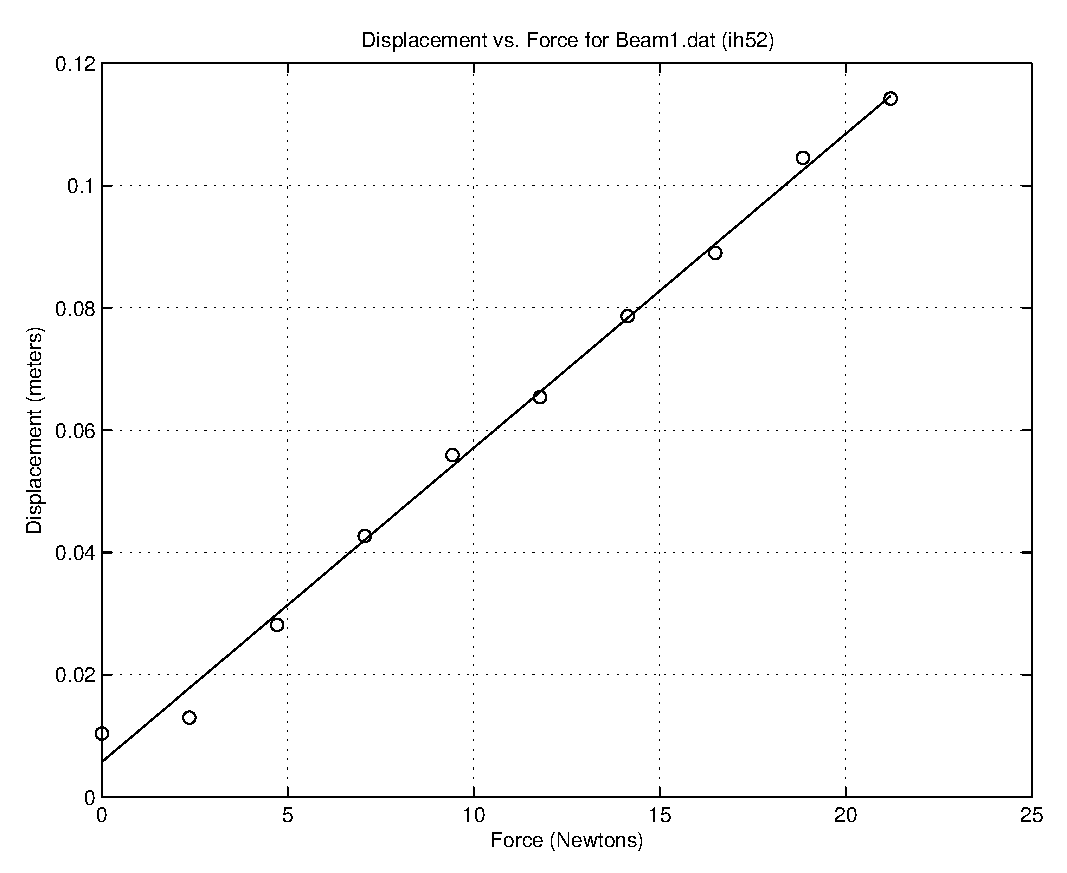
\epsfig{file=Beam1Plot.eps, width=3.5in}
\caption{Displacement vs. Force for Beam 1}
\end{center}
\end{figure}

\begin{figure}[htb]
\begin{center}
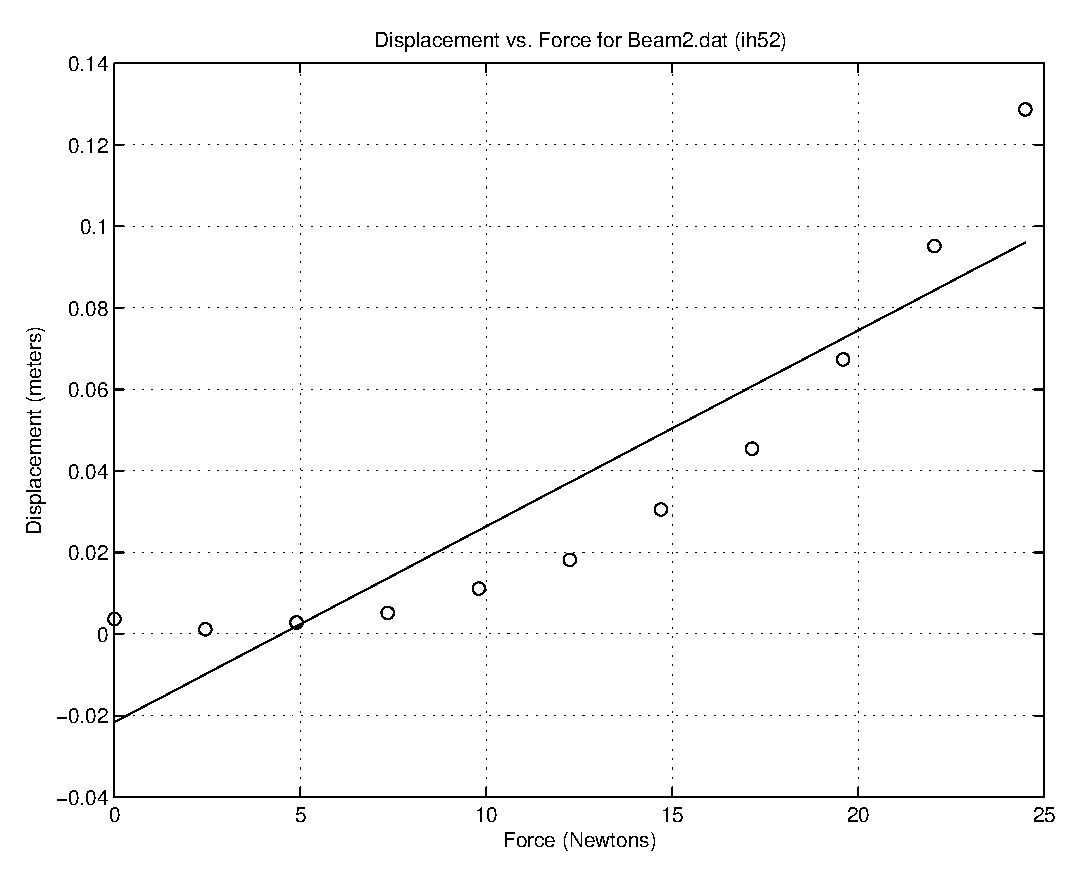
\epsfig{file=Beam2Plot.eps, width=3.5in}
\caption{Displacement vs. Force for Beam 2}
\end{center}
\end{figure}

\begin{figure}[htb]
\begin{center}
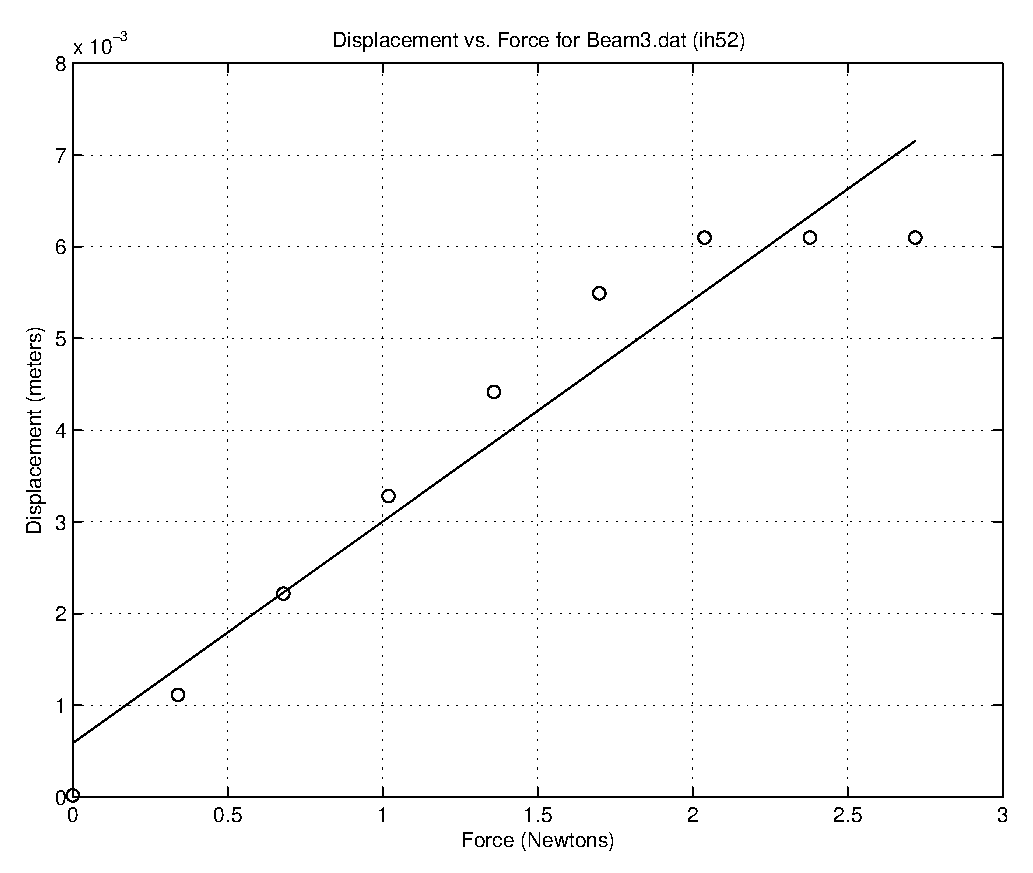
\epsfig{file=Beam3Plot.eps, width=3.5in}
\caption{Displacement vs. Force for Beam 3}
\end{center}
\end{figure}
\end{document}
